\section{Entwurfsänderungen}

Der grundlegende Entwurf hat sich seit der Entwurfsphase nicht geändert. Als im Laufe der Implementierung jedoch die Anforderungen an das Softwareprodukt noch klarer wurden, kamen kleinere Ergänzungen hinzu. Auch die zuvor beschriebenen Probleme bei der Entwicklung führten zu einigen Änderungen.

Die wichtigsten Änderungen sind hier aufgeführt:

\begin{itemize}
\item Einführung eines neuen Unterpakets von View namens CustomComponents, das die Klassen und GUI-Forms der nun ausgelagerten Tabs enthält.

\item Abbildung von Mehrfachinitialisierungen wurde angepasst.

\item Views kennen ihre Parent-View, d.h. Fenster wissen, von welchem Fenster sie erstellt wurden.

\item Es findet keine strikte Unterscheidung zwischen kombinierten Strategien und gemischten Strategien statt. Stattdessen wird das Entwurfsmuster \emph{Kompositum} verwendet.

\item VMResult wurde um die Klasse VMAgentHistory ergänzt. VMAgentHistory beinhaltet Informationen über den Zustand eines Agenten während der Simulation. 

\end{itemize}

\begin{figure}[H]
	\centering
	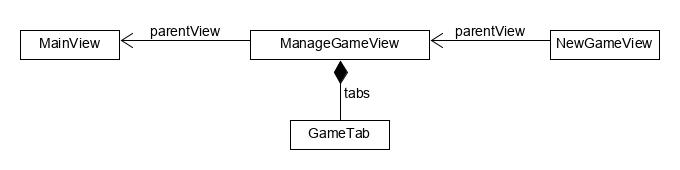
\includegraphics[scale=0.5]{pse_update1.jpg}
	\caption{Anpassung des GUI-Entwurfs. Die Änderungen gelten analog für alle anderen Klassen in der GUI.}
\end{figure}

\begin{figure}[H]
	\centering
	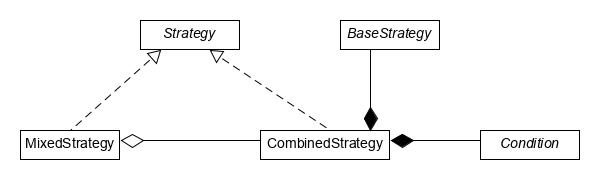
\includegraphics[scale=0.5]{pse_update2.jpg}
	\caption{Kompositum Entwurfsmuster für Strategien.}
\end{figure}